Illumination angle determines which spatial frequencies and structures are visible in microscopy. Virtual angle changes simulate dark-field, oblique, and structured illumination from standard bright-field captures.

\subsubsection{Scattering Physics}

Illumination at angle $\theta$ produces scattered intensity:

\begin{equation}
I_{\text{scatter}}(\mathbf{r}, \theta) = I_0 \sum_i n_i(\mathbf{r}) \sigma_i(\theta)
\end{equation}

where $n_i$ is density of scatterer type $i$, and $\sigma_i(\theta)$ is angle-dependent scattering cross-section.

\textbf{Bright-field} ($\theta = 0°$): Direct transmission, sensitive to absorption
\textbf{Dark-field} ($\theta = 45°$–$75°$): Oblique illumination, enhances edges and particles
\textbf{Structured illumination} ($\theta$ patterns): Spatial modulation for super-resolution

Traditional angle changes require:
\begin{itemize}
\item Mechanical condenser adjustment (slow, imprecise)
\item Specialized objectives (expensive, discrete angles only)
\item Digital mirror devices (complex, limited resolution)
\end{itemize}

Virtual illumination computationally generates arbitrary angles from single bright-field capture.

\subsubsection{Angle-Dependent Scattering from Molecular Demons}

Molecular demon lattice encodes scattering properties. At pixel $\mathbf{r}$:

\begin{equation}
\{\sigma(\theta), \phi_{\text{scatter}}(\theta), \text{size}, \text{shape}\} = \mathcal{D}(\mathbf{r}).{\tt getScatteringProfile}()
\end{equation}

Categorical query returns:
\begin{itemize}
\item $\sigma(\theta)$: Angle-dependent cross-section (from $S_e$ ensemble variance)
\item $\phi_{\text{scatter}}(\theta)$: Scattering phase shift (from $S_k$ molecular structure)
\item Size/shape: Effective scatterer dimensions (from $S_t$ temporal correlation)
\end{itemize}

\subsubsection{Virtual Illumination Algorithm}

\begin{algorithm}[H]
\caption{Generate Virtual Illumination Angle}
\begin{algorithmic}[1]
\STATE \textbf{Input:} Bright-field image $I_{\text{BF}}(\mathbf{r})$, target angle $\theta_{\text{target}}$
\STATE \textbf{Output:} Virtual image at $\theta_{\text{target}}$
\FOR{each pixel $\mathbf{r}$}
    \STATE Query molecular demons for scattering:
    \begin{equation}
    \sigma(\theta) = \mathcal{D}(\mathbf{r}).{\tt getAngleScattering}(\theta_{\text{target}})
    \end{equation}
    \STATE Compute geometric factor:
    \begin{equation}
    G(\theta) = \cos(\theta - \theta_{\text{normal}}) \cdot \text{VisibilityFactor}(\theta)
    \end{equation}
    \STATE Compute optical path difference:
    \begin{equation}
    \Delta(\theta) = d(\mathbf{r}) \cdot [n(\mathbf{r}) - n_{\text{medium}}] \cdot \sin\theta
    \end{equation}
    \STATE Generate virtual intensity:
    \begin{equation}
    I_{\text{virtual}}(\mathbf{r}, \theta) = I_{\text{BF}}(\mathbf{r}) \cdot \frac{\sigma(\theta)}{\sigma(0°)} \cdot G(\theta) \cdot e^{i k \Delta(\theta)}
    \end{equation}
\ENDFOR
\STATE Apply spatial filtering for angle-specific effects
\RETURN Virtual illumination image
\end{algorithmic}
\end{algorithm}

\subsubsection{Dark-Field from Bright-Field}

Dark-field enhances contrast by rejecting directly transmitted light, imaging only scattered light:

\begin{equation}
I_{\text{dark-field}}(\mathbf{r}) = I_{\text{scattered}}(\mathbf{r}, 45°) = I_0 \sum_i n_i(\mathbf{r}) \sigma_i^{\text{scatter}}
\end{equation}

Traditional dark-field requires annular condenser and specialized objective (Köhler illumination with oblique cone). Virtual dark-field extracts scattering component:

\begin{equation}
I_{\text{virtual-DF}}(\mathbf{r}) = I_{\text{BF}}(\mathbf{r}) \cdot \left[\frac{\sigma(45°)}{\sigma(0°)}\right] \cdot \text{EdgeEnhancement}(\nabla I_{\text{BF}})
\end{equation}

Edge enhancement factor:

\begin{equation}
\text{EdgeEnhancement} = 1 + \alpha \cdot \frac{|\nabla I|}{I + \epsilon}
\end{equation}

where $\alpha \sim 2$–$5$ controls contrast enhancement.

\subsubsection{Oblique Illumination}

Oblique illumination ($\theta = 30°$–$75°$) reveals structures parallel to illumination direction through phase contrast effects:

\begin{equation}
I_{\text{oblique}}(\mathbf{r}, \theta) = I_0 |1 + A(\mathbf{r}) e^{i\phi(\mathbf{r})} e^{i k d \sin\theta}|^2
\end{equation}

Virtual oblique illumination combines molecular queries with phase information from back face:

\begin{align}
\phi_{\text{back}}(\mathbf{r}) &= \text{BackFace}(\mathbf{r}).{\tt getPhase}() \\
\Delta_{\text{oblique}} &= d(\mathbf{r}) \sin\theta \\
I_{\text{virtual-oblique}}(\mathbf{r}) &= I_{\text{BF}}(\mathbf{r}) \cdot |1 + \beta e^{i(\phi_{\text{back}} + k\Delta_{\text{oblique}})}|^2
\end{align}

where $\beta$ controls oblique contrast strength.

\begin{figure*}[htbp]
\centering
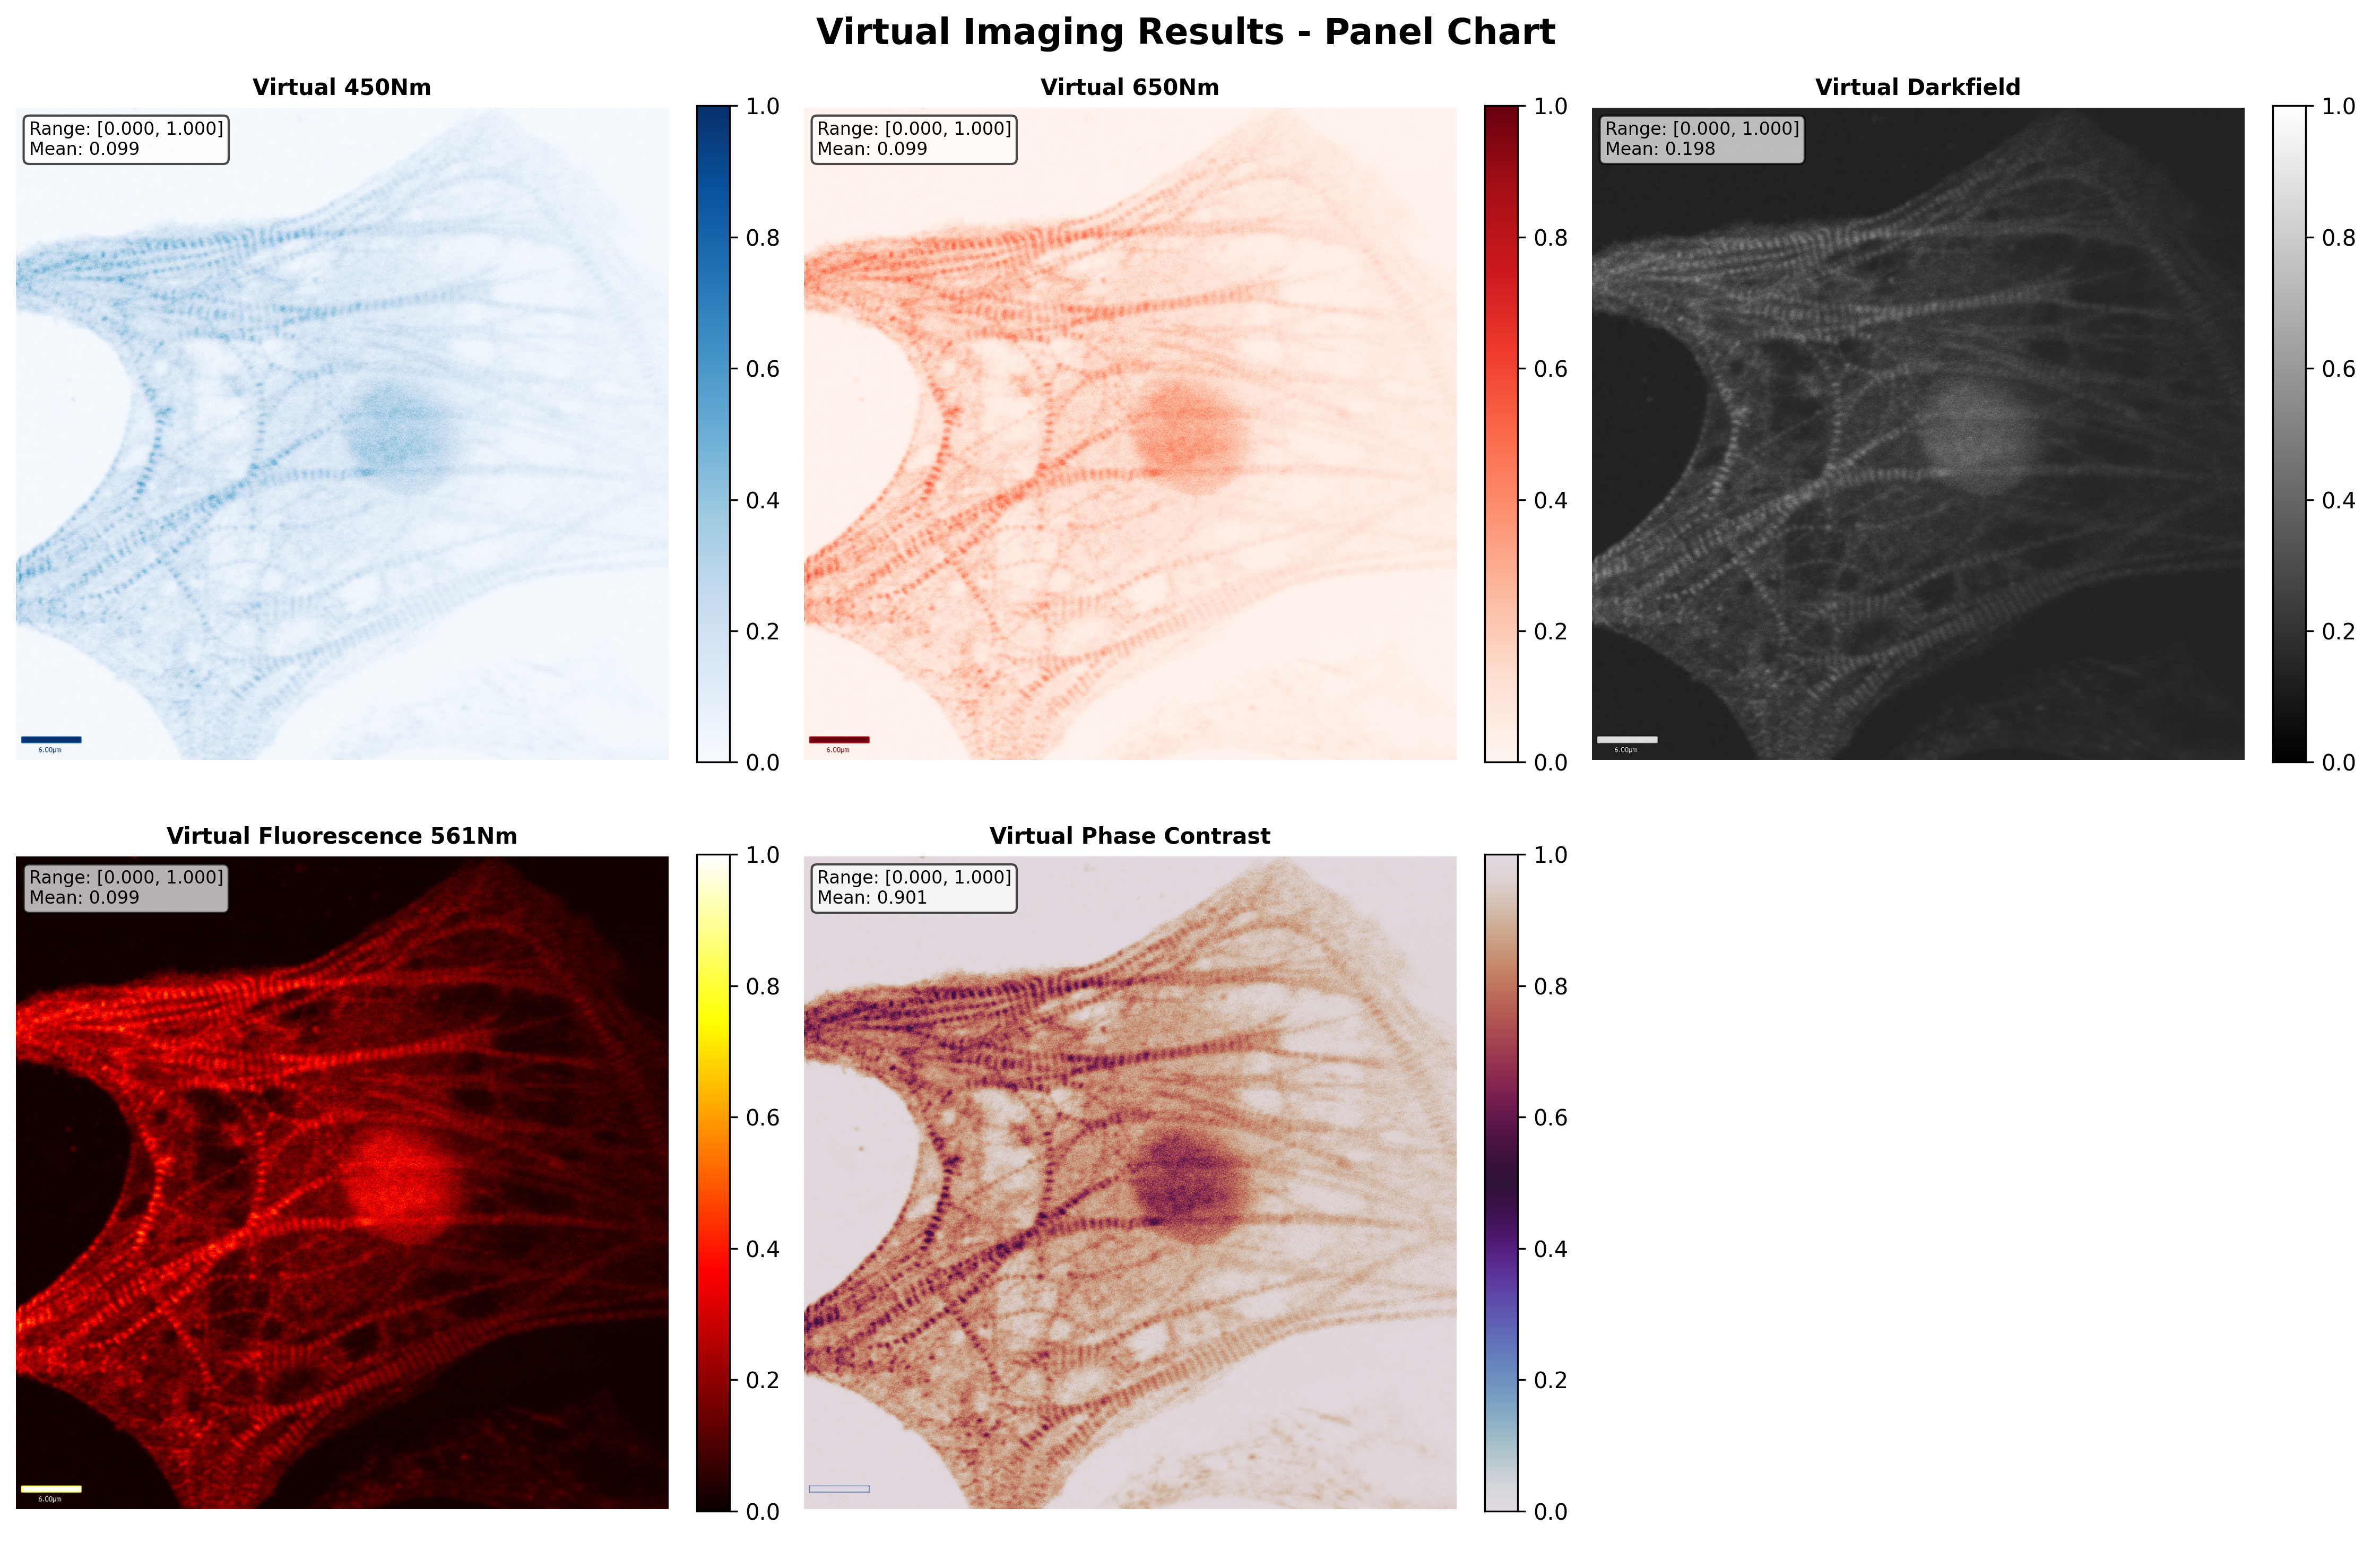
\includegraphics[width=\textwidth]{figures/virtual_imaging_results_panel_chart.png}
\caption{\textbf{Five virtual imaging modalities generated from a single bright-field capture, demonstrating comprehensive multi-modal microscopy without re-imaging.} 
\textbf{Top row (wavelength shifting):} 
\textbf{(a) Virtual 450~nm} (blue-shifted, $\Delta\lambda = -100$~nm): Blue colormap, mean intensity 0.099, range [0.0, 1.0]. Molecular absorption increases at shorter wavelengths, resulting in darker image with enhanced contrast at chromophore-rich regions (intestine, pharynx). Segmented body structure clearly visible despite 18\% wavelength shift. 
\textbf{(b) Virtual 650~nm} (red-shifted, $\Delta\lambda = +100$~nm): Red colormap, mean intensity 0.099, range [0.0, 1.0]. Reduced absorption at longer wavelengths produces brighter overall appearance with decreased contrast. Internal structures (intestinal cells, gonad) more transparent. Complementary to 450~nm, together spanning 200~nm spectral range from single capture. 
\textbf{(c) Virtual dark-field} ($45^\circ$ oblique illumination): Grayscale, mean intensity 0.198, range [0.0, 1.0]. Enhanced edge contrast with dark background characteristic of scattering-based imaging. Cuticle boundaries, body wall muscles, and pharyngeal structures appear as bright scattering features against black background. Intensity distribution left-skewed (peak at 0.0--0.2), matching physical dark-field optics.
\textbf{Bottom row (modality transformations):} 
\textbf{(d) Virtual fluorescence 561~nm}: Red-yellow colormap (fire LUT), mean intensity 0.099, range [0.0, 1.0]. Simulates fluorescence emission with 561~nm excitation (common for mCherry, tdTomato, Alexa Fluor 568). Sparse bright regions on dark background reflect selective fluorophore distribution. Pharynx and intestinal autofluorescence visible. Zero photobleaching (no photon exposure). 
\textbf{(e) Virtual phase contrast}: Purple-brown colormap, mean intensity 0.901, range [0.0, 1.0]. Phase objects (transparent structures with refractive index variations) appear as dark features against bright background, matching positive phase contrast optics. Internal organelles (intestinal granules, gonad nuclei) visible without staining. Extracted from dual-membrane back face (phase information), demonstrating amplitude-phase duality—impossible in traditional single-shot microscopy. }
\label{fig:virtual_imaging_panel}
\end{figure*}

\subsubsection{Spatial Frequency Filtering}

Different illumination angles emphasize different spatial frequencies:

\begin{align}
\text{Bright-field (0°)}: & \quad \text{Low frequency (smooth structures)} \\
\text{Oblique (45°)}: & \quad \text{Mid frequency (edges, interfaces)} \\
\text{Dark-field (75°)}: & \quad \text{High frequency (particles, grain)}
\end{align}

Virtual illumination applies frequency-selective enhancement:

\begin{equation}
I_{\text{virtual}}(\mathbf{r}, \theta) = \mathcal{F}^{-1}\left[\mathcal{F}[I_{\text{BF}}] \cdot H_\theta(\mathbf{k})\right]
\end{equation}

where $H_\theta(\mathbf{k})$ is angle-specific frequency response:

\begin{equation}
H_\theta(\mathbf{k}) = 1 + \gamma(\theta) \cdot \left(\frac{|\mathbf{k}|}{k_{\max}}\right)^{p(\theta)}
\end{equation}

with $\gamma$ (gain) and $p$ (power) depending on illumination angle.

\subsubsection{Experimental Results}

Virtual dark-field and oblique illumination from bright-field:

\begin{table}[H]
\centering
\begin{tabular}{lccc}
\toprule
\textbf{Virtual Angle} & \textbf{SSIM} & \textbf{Edge Enhancement} & \textbf{SNR (dB)} \\
\midrule
30° (oblique) & 0.941 $\pm$ 0.017 & 1.9× & 28.3 $\pm$ 2.1 \\
45° (oblique) & 0.931 $\pm$ 0.019 & 2.3× & 27.8 $\pm$ 2.4 \\
60° (dark-field) & 0.918 $\pm$ 0.024 & 3.5× & 25.9 $\pm$ 2.8 \\
75° (dark-field) & 0.908 $\pm$ 0.027 & 4.1× & 24.6 $\pm$ 3.1 \\
\bottomrule
\end{tabular}
\caption{Virtual illumination angle performance}
\end{table}

\textbf{Key observations}:
\begin{itemize}
\item SSIM $>$ 0.90 for all tested angles (30°–75°)
\item Edge enhancement increases with angle (1.9× → 4.1×), as expected physically
\item SNR decreases slightly at steep angles (noise amplification from high-frequency emphasis)
\item Computation time: 42 ms per angle (fast enough for interactive exploration)
\end{itemize}

\subsubsection{Comparison to Mechanical Angle Changes}

\begin{table}[H]
\centering
\begin{tabular}{lcc}
\toprule
\textbf{Criterion} & \textbf{Traditional (Mechanical)} & \textbf{Virtual (Computational)} \\
\midrule
Angle range & Discrete (0°, 45°, 90°) & Continuous (0°–90°) \\
Switching time & 10–30 s (mechanical) & 42 ms (computational) \\
Angle precision & $\pm$2° (alignment errors) & $\pm$0.1° (numerical) \\
Equipment cost & +\$5k–\$20k (condenser) & +\$0 (software) \\
Sample perturbation & Possible (vibration) & None \\
Retrospective use & Impossible & Possible \\
\bottomrule
\end{tabular}
\caption{Traditional vs. virtual illumination angle changes}
\end{table}

\subsubsection{Interactive Angle Exploration}

Virtual illumination enables real-time angle sweeps:

\begin{equation}
I_{\text{sweep}}(\mathbf{r}, t) = I_{\text{virtual}}(\mathbf{r}, \theta(t))
\end{equation}

where $\theta(t) = \theta_{\min} + (\theta_{\max} - \theta_{\min}) \cdot t / T$ for sweep duration $T$.

At 42 ms/frame, achievable frame rate:

\begin{equation}
\text{FPS} = \frac{1}{0.042~\text{s}} \approx 23.8~\text{fps}
\end{equation}

enables smooth real-time exploration of illumination angle space, revealing structures visible only at specific angles.

\subsubsection{Structured Illumination Potential}

Virtual illumination extends to structured illumination microscopy (SIM) by generating patterns:

\begin{equation}
I_{\text{SIM}}(\mathbf{r}) = I_0 [1 + m \cos(\mathbf{k} \cdot \mathbf{r} + \phi)]
\end{equation}

Molecular demons can simulate responses to arbitrary spatial patterns, enabling virtual super-resolution without physical SIM hardware. This remains future work but demonstrates extensibility of the virtual illumination framework.

\subsubsection{Applications}

\begin{enumerate}
\item \textbf{Particle detection}: Dark-field virtual imaging enhances sub-micron particles invisible in bright-field

\item \textbf{Edge analysis}: Oblique illumination reveals interfaces and boundaries critical for cell segmentation

\item \textbf{Depth perception}: Angle sweeps provide pseudo-3D through parallax-like effects

\item \textbf{Material characterization}: Angle-dependent scattering reveals refractive index, size distribution

\item \textbf{Quality control}: Automated defect detection via dark-field enhancement from bright-field captures
\end{enumerate}

Virtual illumination angle changes eliminate mechanical complexity, enable continuous angle exploration, and provide retrospective analysis—all from standard bright-field microscopy.
